% !TeX root=../main.tex

\chapter*{پاسخ پروژه بخش سوم}
\section*{ پاسخ سوال یک، محاسبه دینامیک وارون در شبیه ساز}

در این بخش، برای شبیه سازی دینامیک وارون سیستم باید مقادیر فضای کاری به سیستم داده شده و مقادیر گشتاور مفاصل اندازه گیری شود. برای این منظور، با اعمال ورودی به مفاصل در قالب زاویه و اندازه گیری گشتاور تولید شده در هر مفصل، می توانیم دینامیک وارون سیستم را شبیه سازی کنیم. دیاگرام سیستم در این قسمت به صورت صورت زیر طراحی می شود.
\begin{figure}[H]
	\centering
	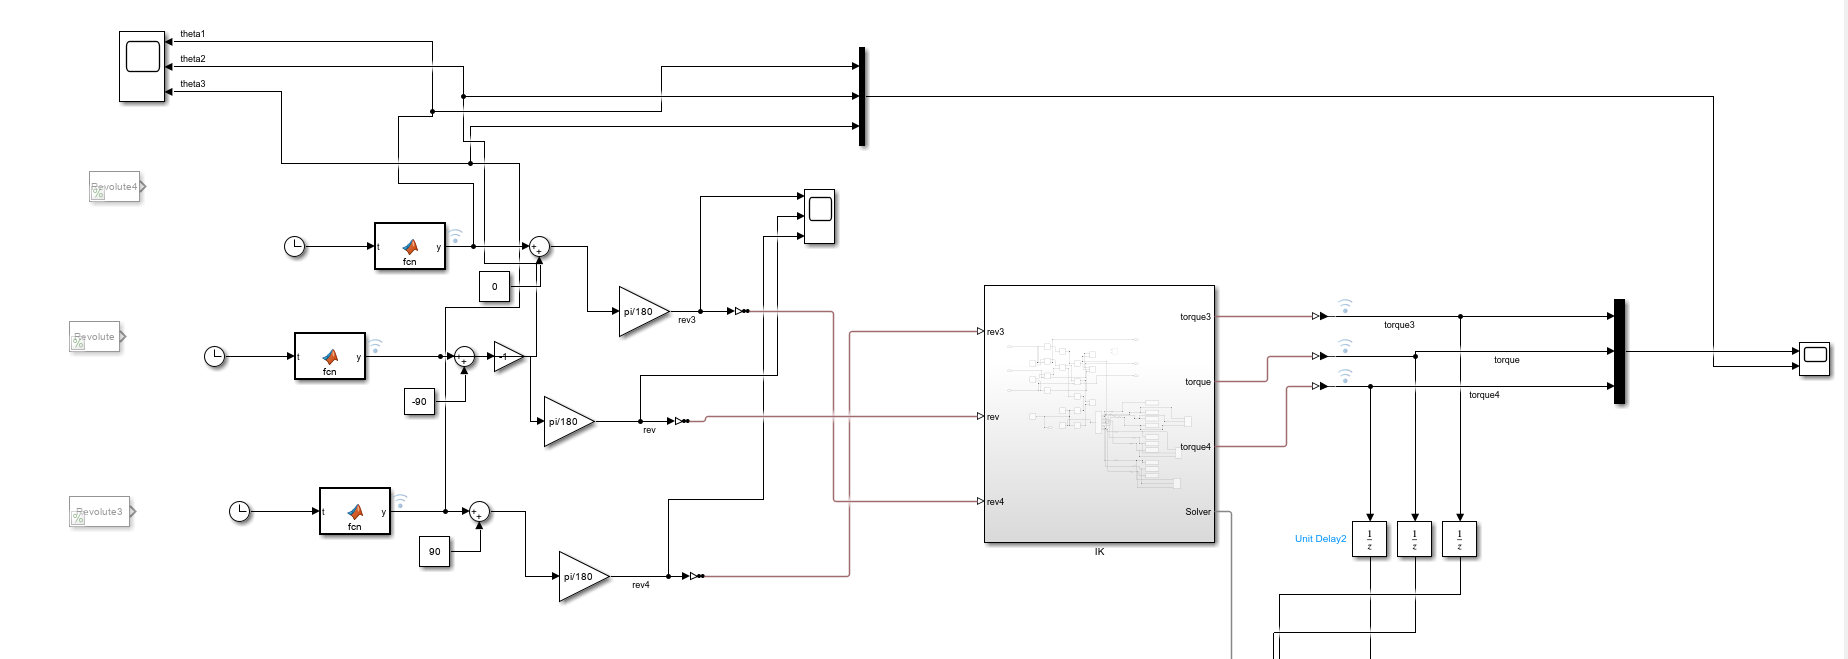
\includegraphics[width=1\linewidth]{../img/1}
	\caption{دیاگرام دینامیک وارون}
	\label{fig:1}
\end{figure}
در این دیاگرام، زوایای سینوسی ورودی بر حسب زمان در ورودی به سیستم وارد می شود. این سیگنال های ورودی در تصویر زیر نمایش داده شده است.
\begin{figure}[H]
	\centering
	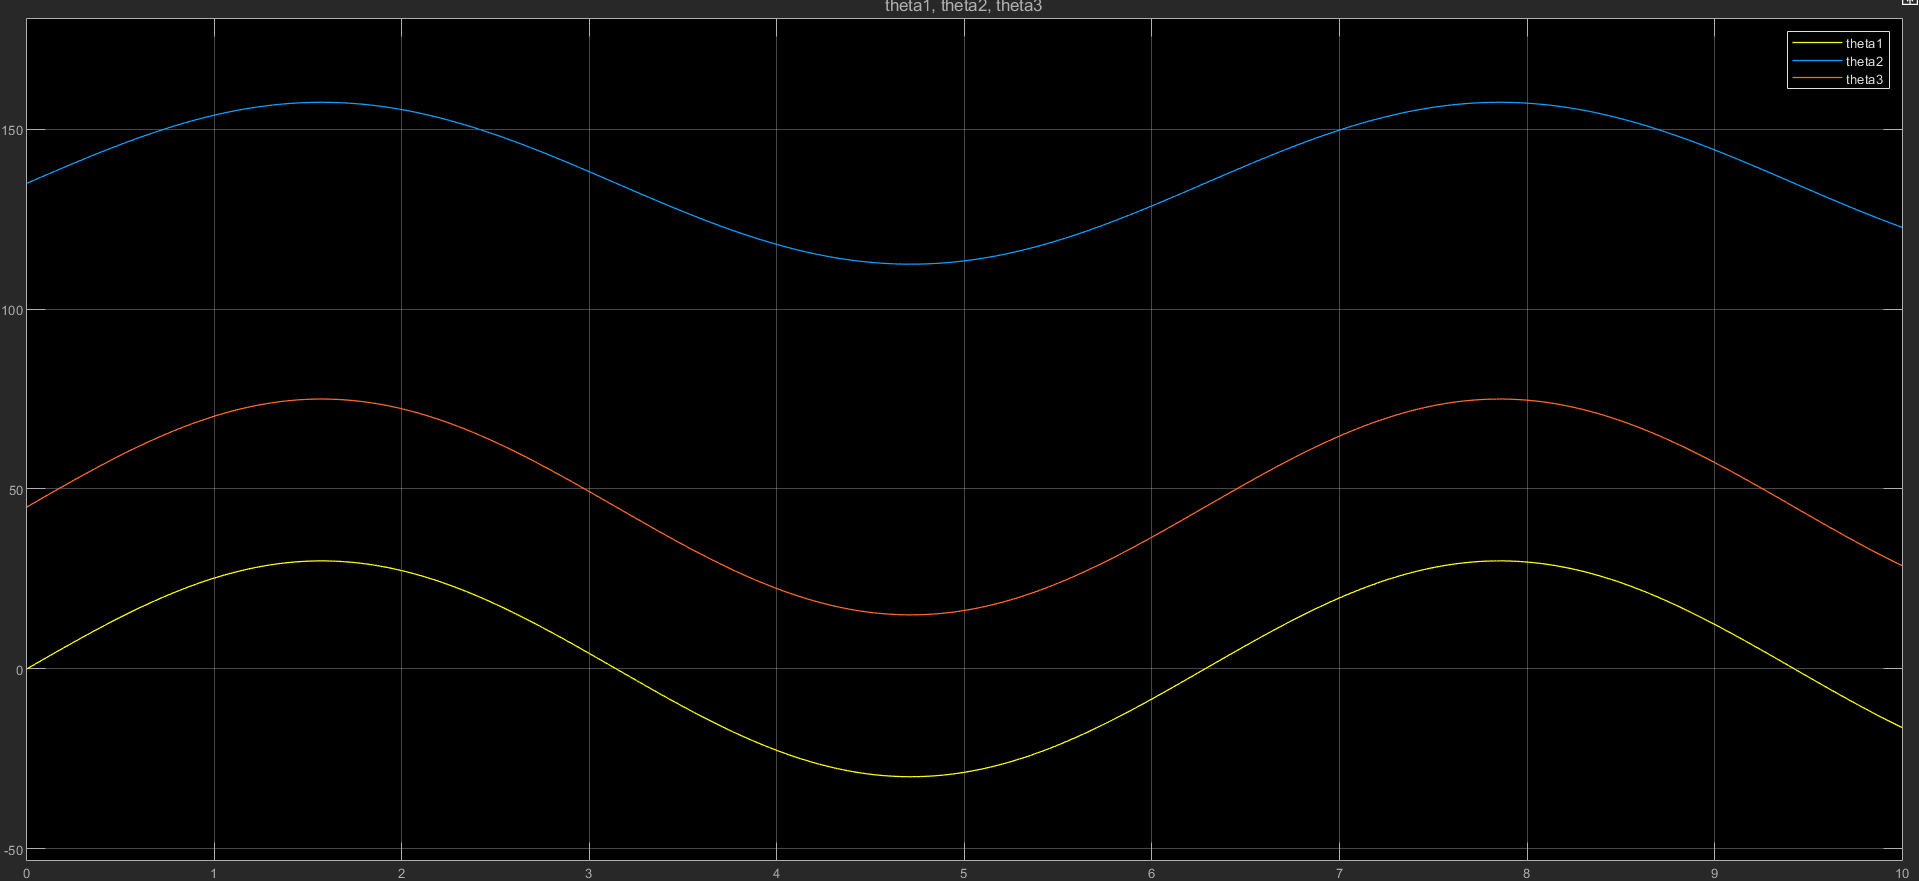
\includegraphics[width=1\linewidth]{../img/2}
	\caption{ورودی های سینوسی به سیستم}
	\label{fig:2}
\end{figure}
در ادامه، برای تبدیل زوایای ورودی به سیستم به رادیان و همچنین تطابق زوایای ابتدایی سیستم، با استفاده از دو بلوک بهره و بایاس این مقادیر مشخص می شود. 
این مقادیر ورودی در بخش بعد به بلوک دینامیک وارون سیستم وارد می شود که در تصویر زیر نمایش داده شده است.
\begin{figure}[H]
	\centering
	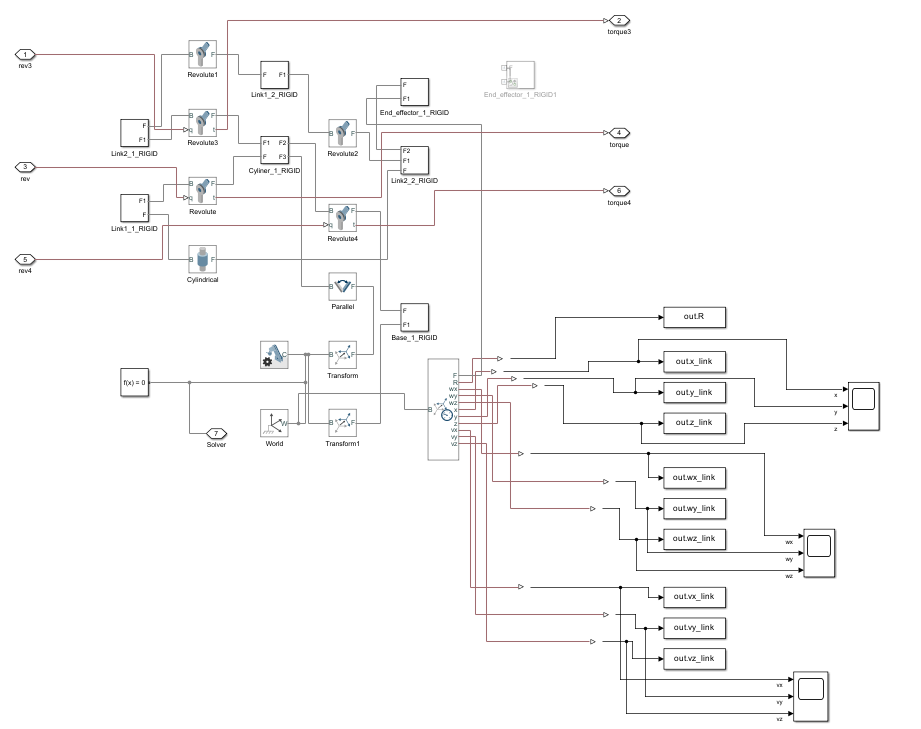
\includegraphics[width=1\linewidth]{../img/3}
	\caption{دیاگرام دینامیک وارون}
	\label{fig:3}
\end{figure}
در این بلوک، مقادیر ورودی به بلوک های revolute به عنوان ورودی های مفاصل q وارد می کنیم.
برای مشاهده ی گشتاور تولید شده در هر مفصل، سنسور $Actuator Torque$ را فعال می کنیم.
\begin{figure}[H]
	\centering
	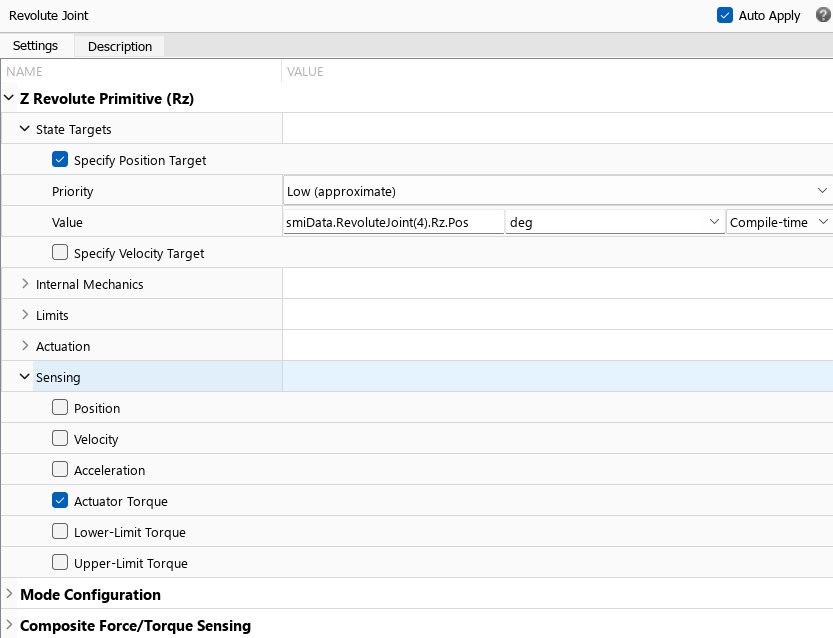
\includegraphics[width=1\linewidth]{../img/4}
	\caption{تنظیمات مفاصل}
	\label{fig:4}
\end{figure}
در پایان این بخش، با اعمال ورودی های مفاصل و بررسی گشتاور تولیدی در هر یک، به بررسی خروجی های به دست آمده برای آنها می پردازیم.
\begin{figure}[H]
	\centering
	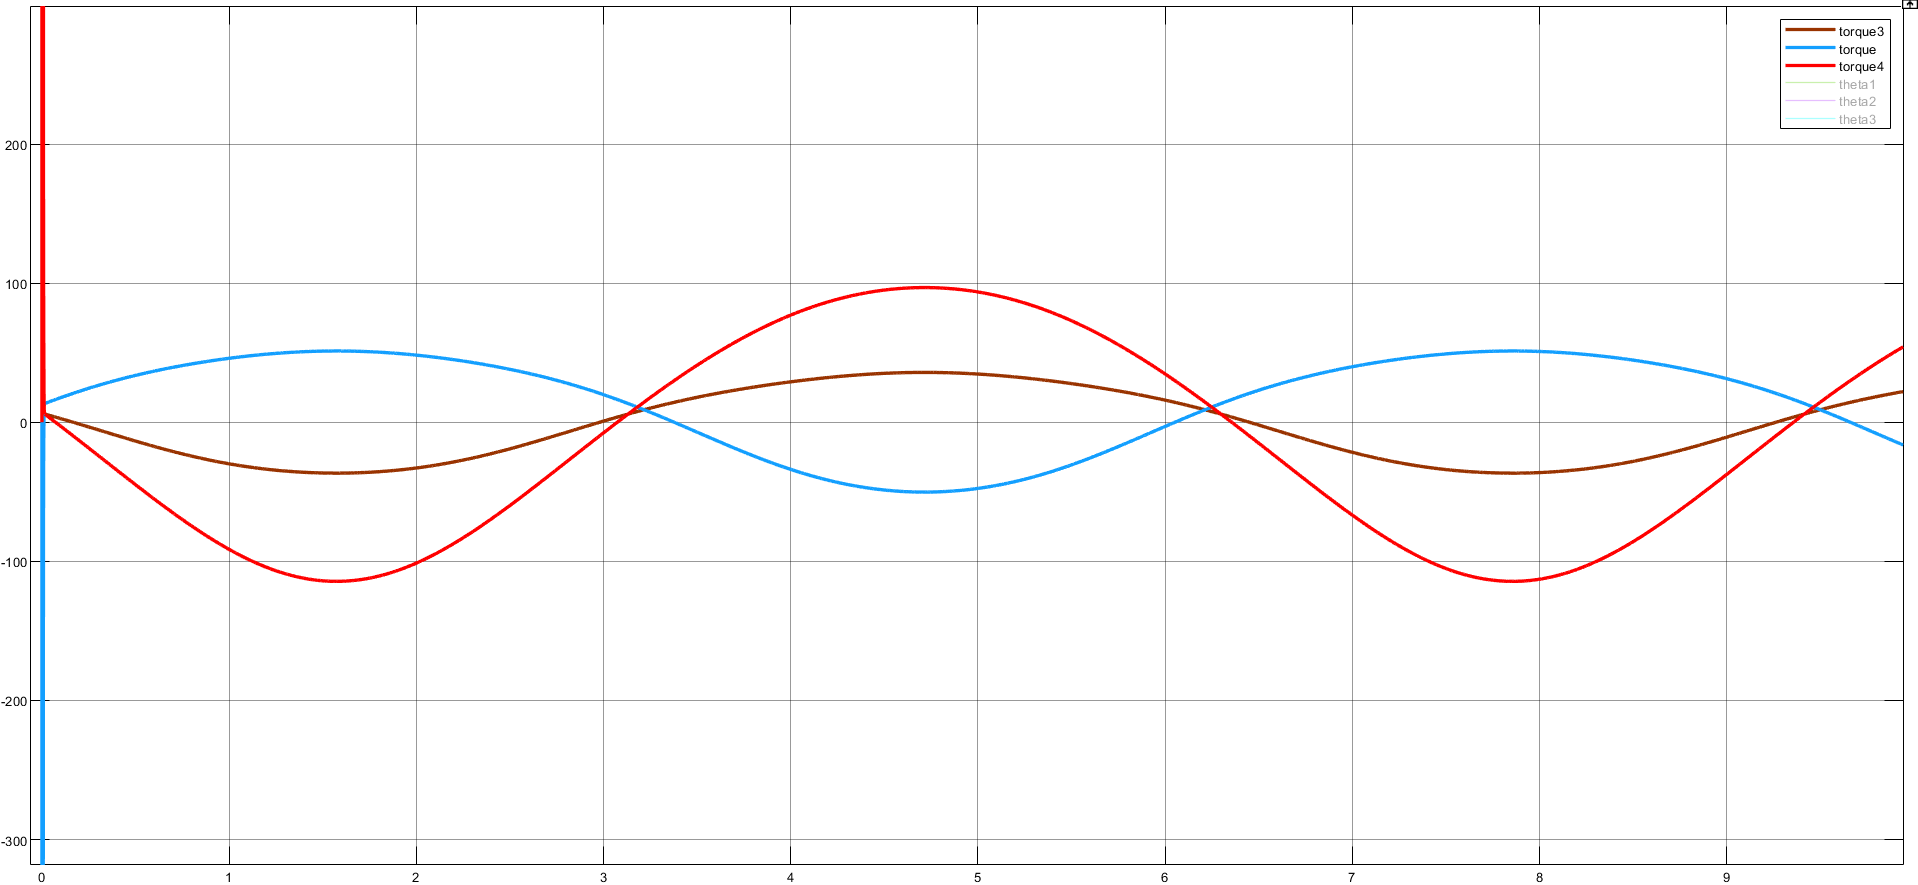
\includegraphics[width=1\linewidth]{../img/5}
	\caption{نمودار گشتاور تولید شده در مفاصل}
	\label{fig:5}
\end{figure}
مشاهده می شود که در لحظات ابتدایی از شبیه سازی، اورشوت زیادی به سیستم اعمال می شود. اما رفتار آن پس از زمان راه اندازی،  پایدار است و مطابق با مسیر های داده شده، خروجی های سینوسی ایجاد می کند. برای بررسی بیشتر و مقایسه ی گشتاور ایجاد شده در هر مفصل با زوایه ی ورودی به آن، می توانیم این سیگنال ها را رسم کنیم.
\begin{figure}[H]
	\centering
	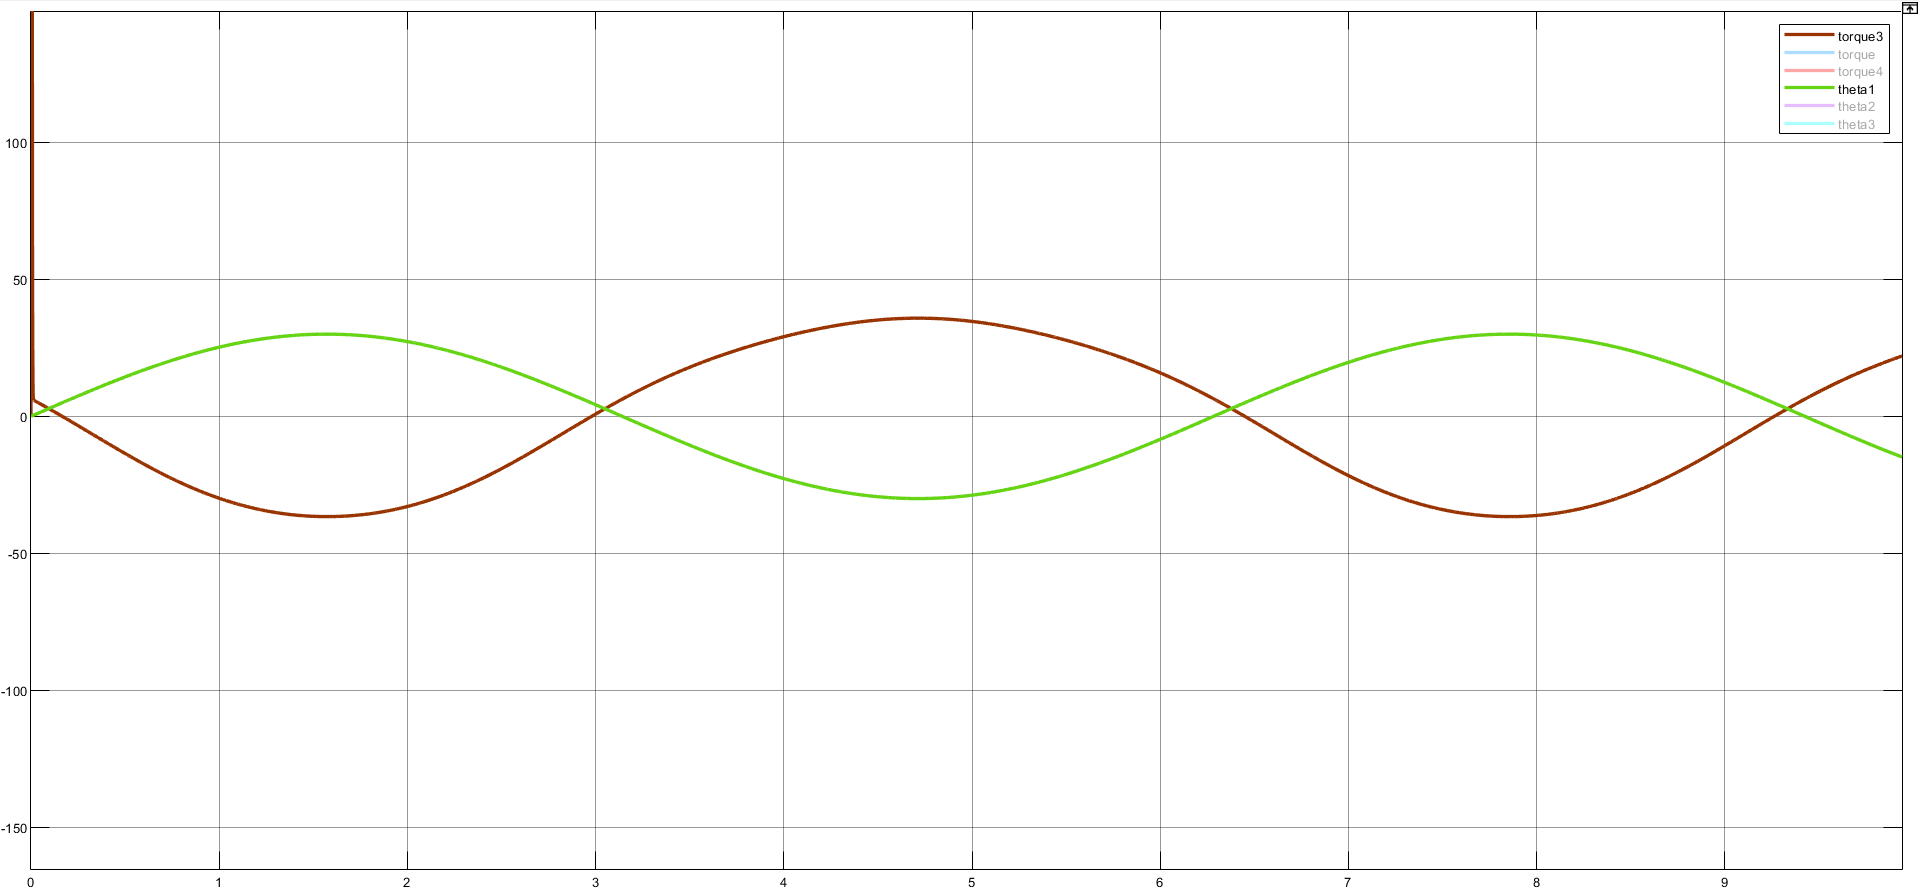
\includegraphics[width=1\linewidth]{../img/6}
	\caption{Theta1}
	\label{fig:6}
\end{figure}
\begin{figure}[H]
	\centering
	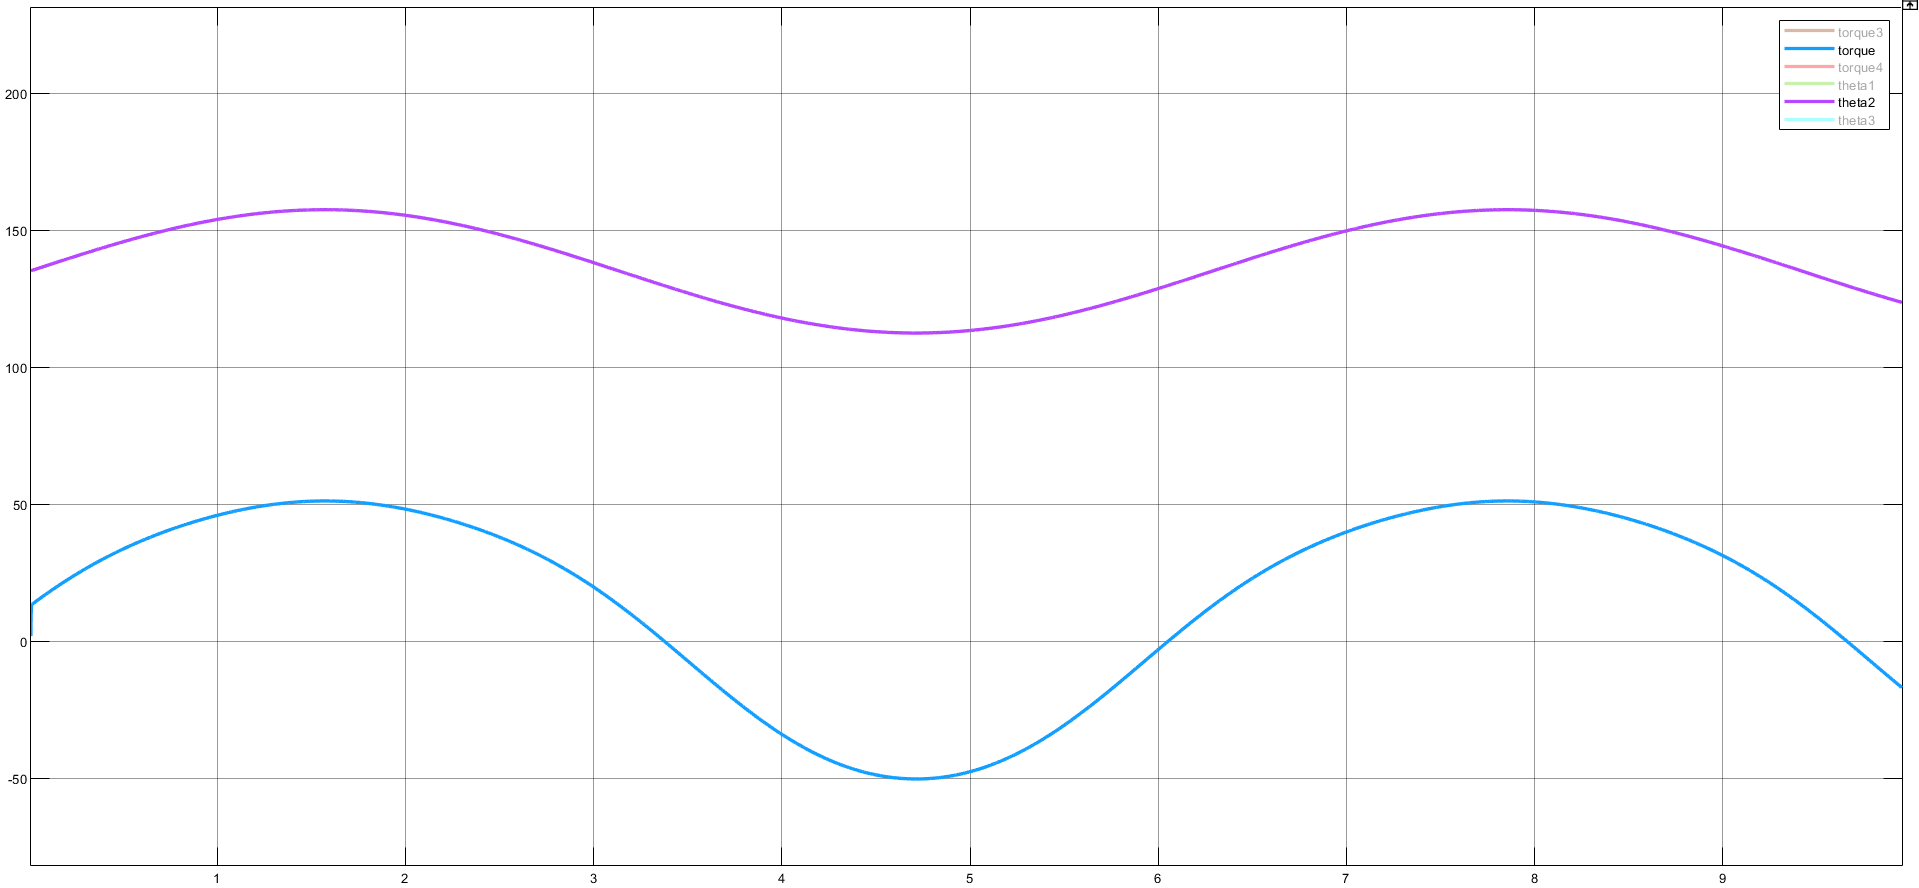
\includegraphics[width=1\linewidth]{../img/7}
	\caption{Theta2}
	\label{fig:7}
\end{figure}
\begin{figure}[H]
	\centering
	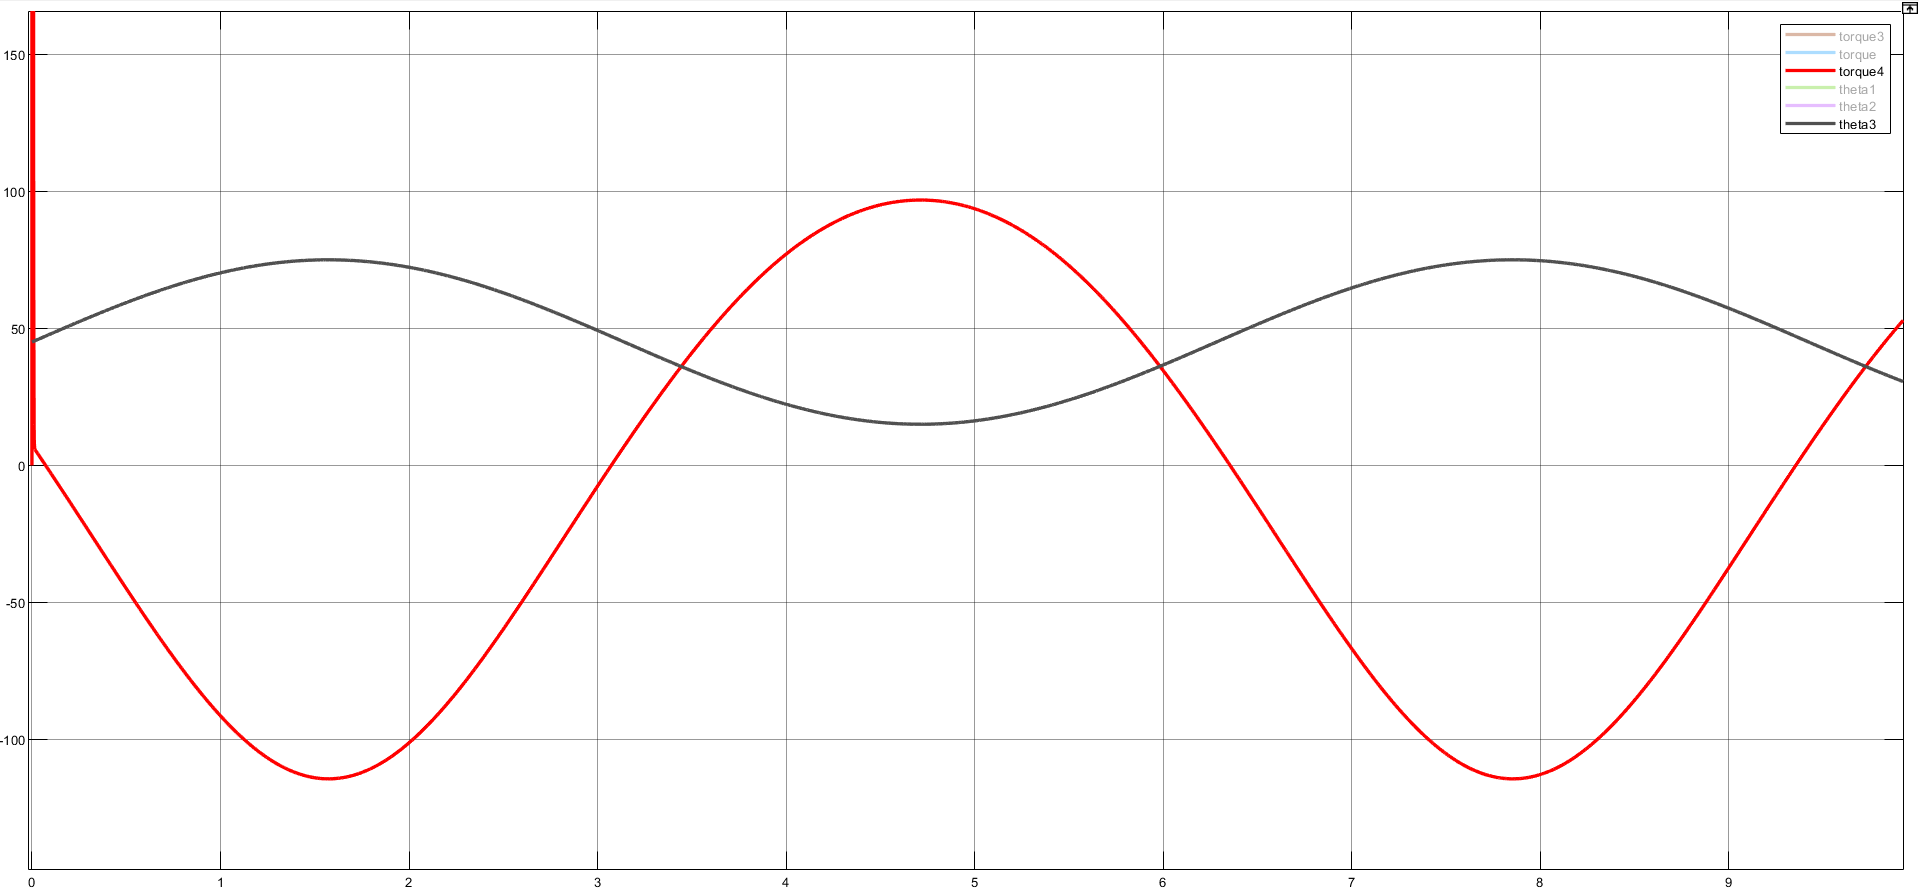
\includegraphics[width=1\linewidth]{../img/8}
	\caption{Theta3}
	\label{fig:8}
\end{figure}
با در نظر داشتن این نمودارها، می توان نتیجه گرفت که بیشترین گشتاور ایجاد شده در هر مفصل در شرایطی است که سرعت  زاویه ای آن $\dot{q}$ برابر صفر شود و مفصل قصد تغییر جهت حرکت داشته باشد.
\section*{ پاسخ سوال دو، محاسبه دینامیک مستقیم در شبیه ساز}
برای محاسبه ی دینامیک مستقیم در شبیه ساز سیستم، لازم است ورودی ها و خروجی های سیستم تغییر داده شوند، به طوری که در این حالت گشتاور ها به عنوان ورودی به مفاصل داده شوند و موقعیت آنها اندازه گیری شود. بنابراین، با تغییر این تنظیمات، می توانیم دینامیک مستقیم ربات را به دست بیاوریم. 
\begin{figure}[H]
	\centering
	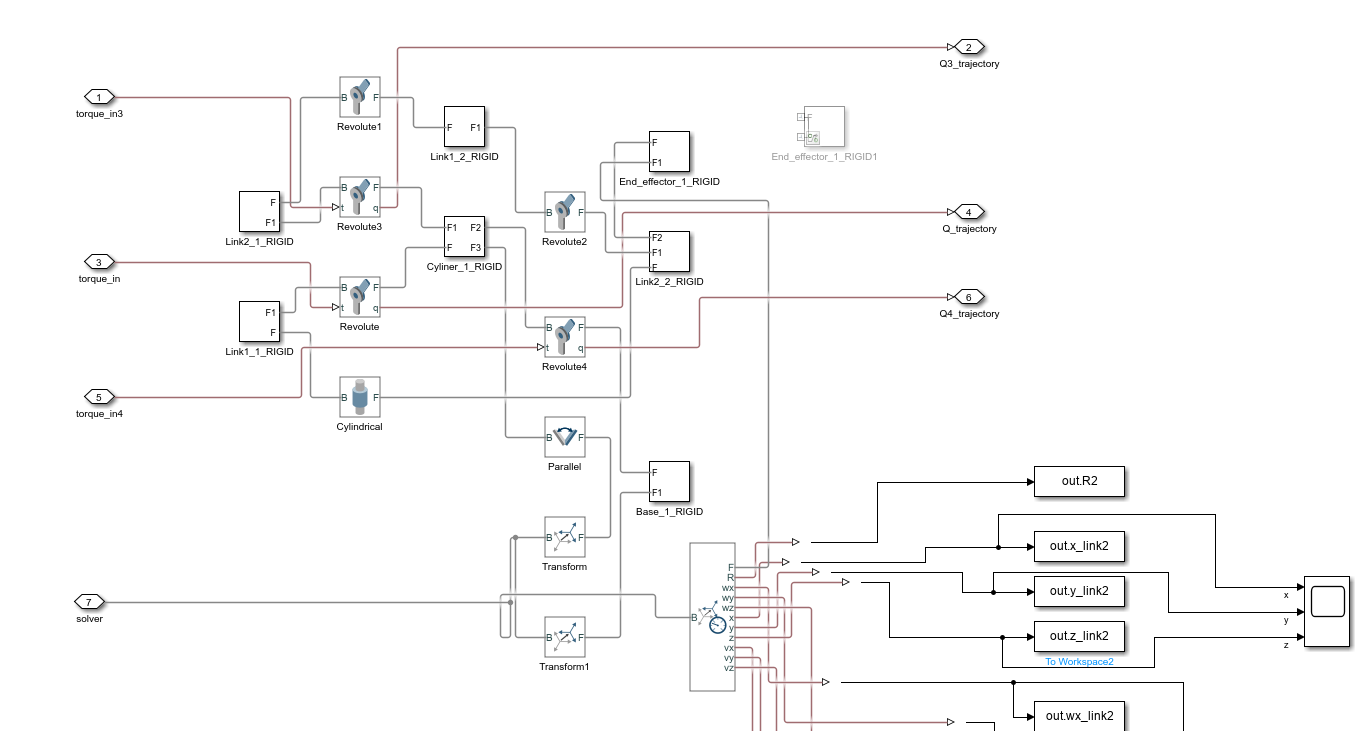
\includegraphics[width=1\linewidth]{../img/9}
	\caption{دیاگرام دینامیک مستقیم}
	\label{fig:9}
\end{figure}
علاوه بر این، برای اجرای همزمان این دو سیستم در یک شبیه سازی، لازم است تا Solver های سیستم دینامیک مستقیم حذف شده و به جای آن، از Solver استفاده شده در بلوک دینامیک وارون استفاده شود. بنابراین، در این بلوک، ورودی دیگری نیز به عنوان Solver طراحی شده است.
ساختار سیستم نهایی در این قسمت به صورت زیر نمایش داده می شود. 
\begin{figure}[H]
	\centering
	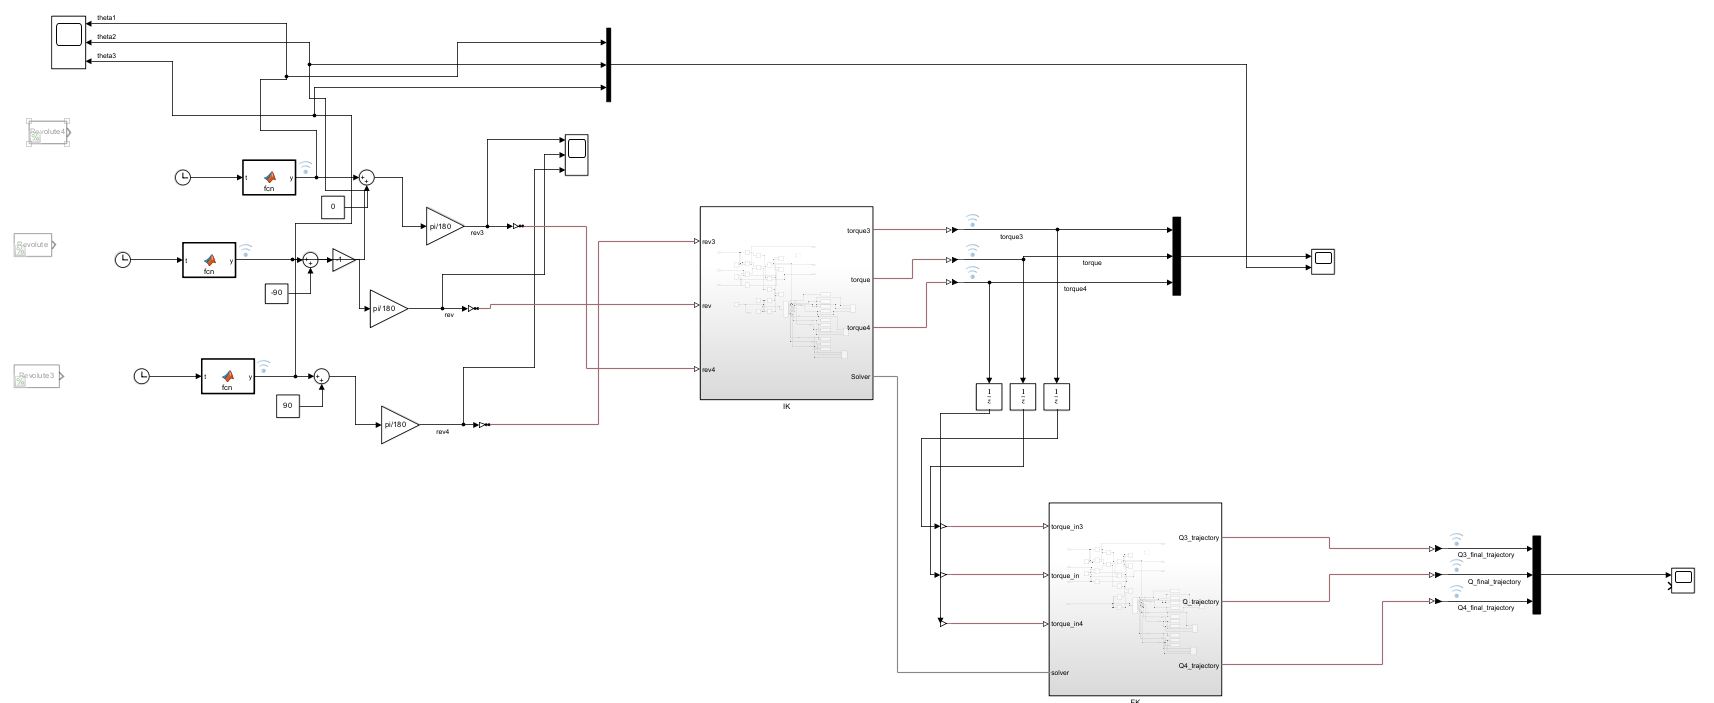
\includegraphics[width=1\linewidth]{../img/10}
	\caption{دیاگرام سیستم با دینامیک مستقیم و وارون}
	\label{fig:10}
\end{figure}
در این سیستم، مقادیر زوایای ورودی در گام اول به بلوک دینامیک وارون وارد شده و با انجام شبیه سازی، گشتاورهای هر مفصل ایجاد می شود. در ادامه، با اعمال این گشتاور ها به بلوک دینامیک مستقیم، مجددا زوایای هر مفصل ایجاد می شود و می توان انتظار داشت که در صورت صحت سیستم های دینامیک مستقیم، نتایج یکسانی در خروجی به دست بیاید.
\section*{ پاسخ سوال سه، طراحی مسیر}
برای ایجاد بلوک طراحی مسیر، مطابق روابط ب.5 و ب.10 کتاب کد تابع متلب نوشته شده و  با وارد کردن مقادیر اولیه و نهایی موقعیت، سرعت و شتاب و همچنین زمان شروع و پایان، مسیر مورد نظر برای هر مفصل ایجاد می شود. 
کد این برنامه در بخش زیر آورده شده است:
\begin{figure}[H]
	\centering
	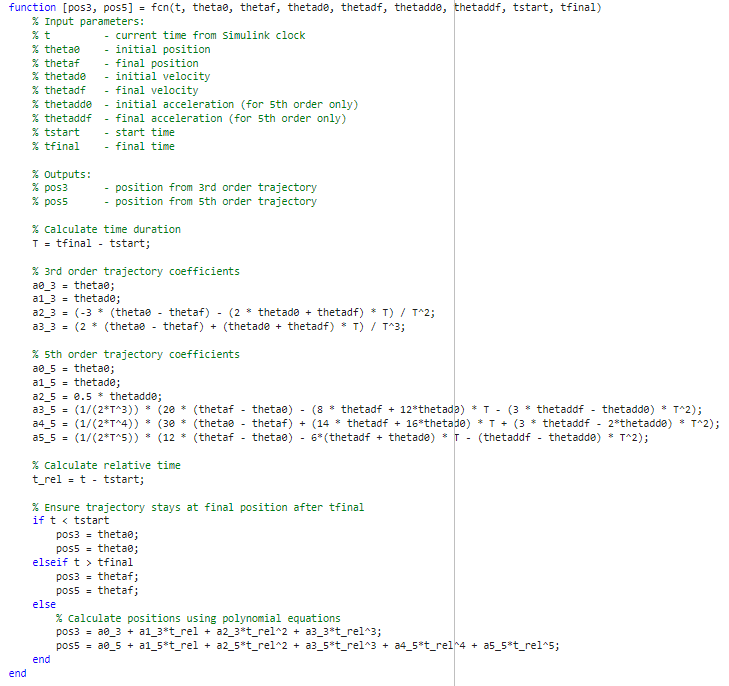
\includegraphics[width=1\linewidth]{../img/11}
	\caption{کد طراحی مسیر}
	\label{fig:11}
\end{figure}
با قرار دادن کد ارائه شده در بلوک $Matlab Function$ و ارائه ی ورودی های مناسب به صورت زیر، می توان مسیر های طراحی شده درجه 3 و 5 را به دست آورد. در تصویر زیر، دیاگرام بلوک طراحی شده نمایش داده شده است.
\begin{figure}[H]
	\centering
	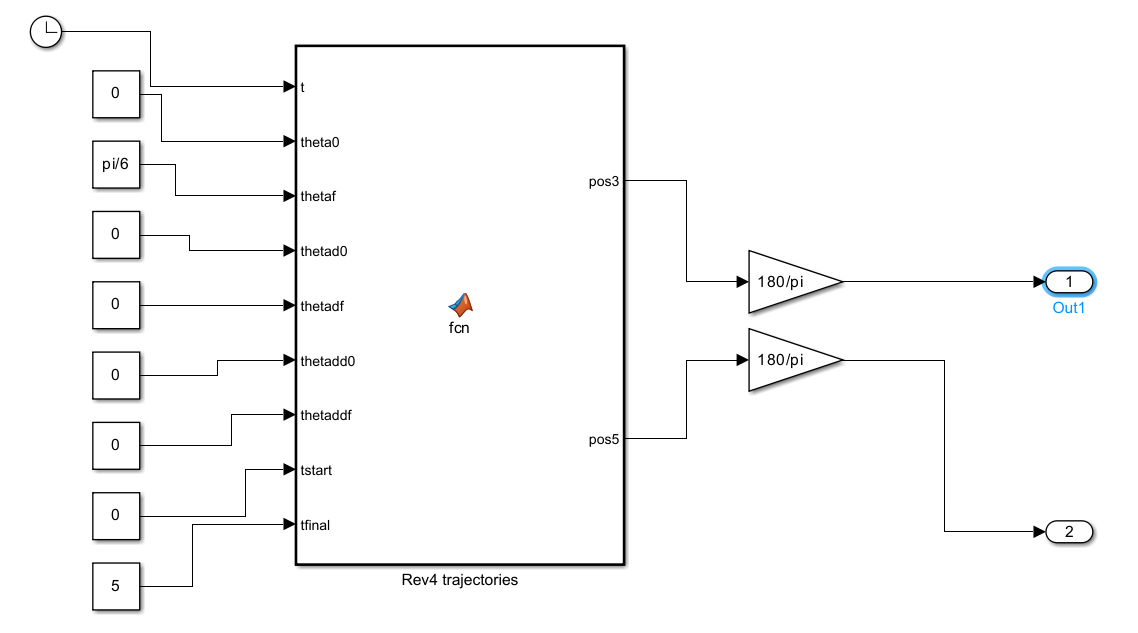
\includegraphics[width=0.7\linewidth]{../img/12}
	\caption{بلوک طراحی مسیر}
	\label{fig:12}
\end{figure}
لازم به ذکر است که مسیر های طراحی شده توسط این بلوک بر حسب رادیان محاسبه می شوند و برای استفاده از آن در ربات، با بلوک های بهره مقادیر به فضای درجه تبدیل شده اند. 
\section*{ پاسخ سوال چهار، طراحی مسیر برای ربات}
با استفاده از بلوک طراحی مسیر در بخش قبل و اعمال ورودی های مشخص شده در تمرین این بخش به شرح زیر، مسیر های خواسته شده را طراحی می کنیم.
\[
t = 0 \, \text{s} \rightarrow t = 5 \, \text{s}, \quad 
\mathbf{q}_0 = \begin{bmatrix} 0 \\ 45 \\ 135 \end{bmatrix} 
\rightarrow \mathbf{q}_f = \begin{bmatrix} 30 \\ 75 \\ 157.5 \end{bmatrix},
\]
\[
\dot{\mathbf{q}}_0 = \begin{bmatrix} 0 \\ 0 \\ 0 \end{bmatrix} 
\rightarrow \dot{\mathbf{q}}_f = \begin{bmatrix} 0 \\ 0 \\ 0 \end{bmatrix},
\]
\[
\ddot{\mathbf{q}}_0 = \begin{bmatrix} 0 \\ 0 \\ 0 \end{bmatrix} 
\rightarrow \ddot{\mathbf{q}}_f = \begin{bmatrix} 0 \\ 0 \\ 0 \end{bmatrix}.
\]

با اعمال ورودی ها به صورت زیر برای بلوک ها خواهیم داشت:
\begin{figure}[H]
	\centering
	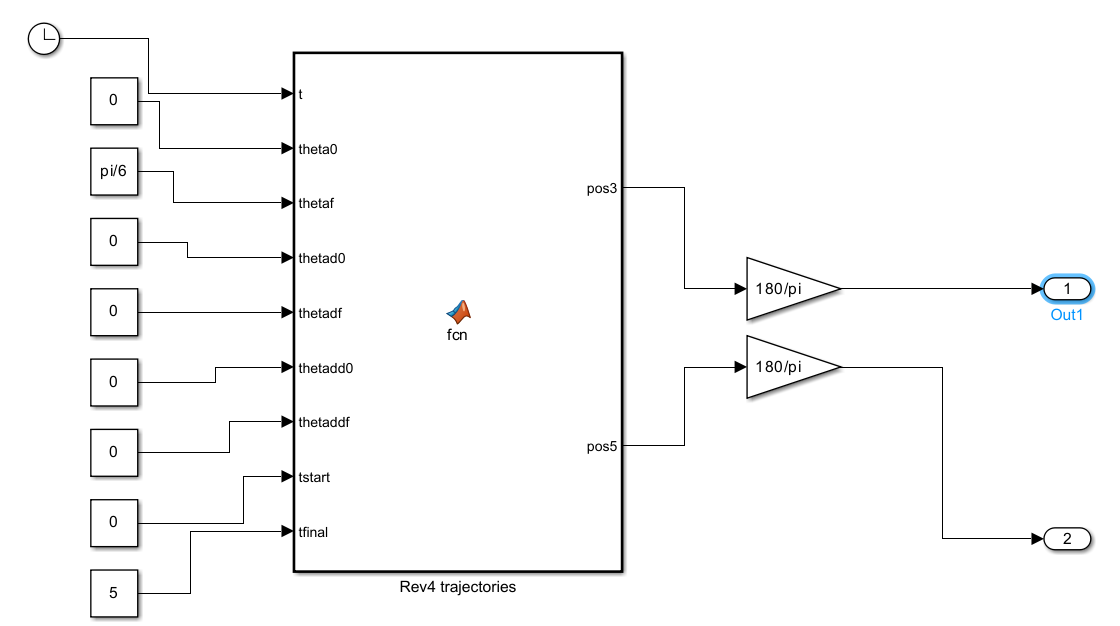
\includegraphics[width=0.7\linewidth]{../img/13}
	\caption{دیاگرام طراحی مسیر مفصل تتا4}
	\label{fig:13}
\end{figure}
\begin{figure}[H]
	\centering
	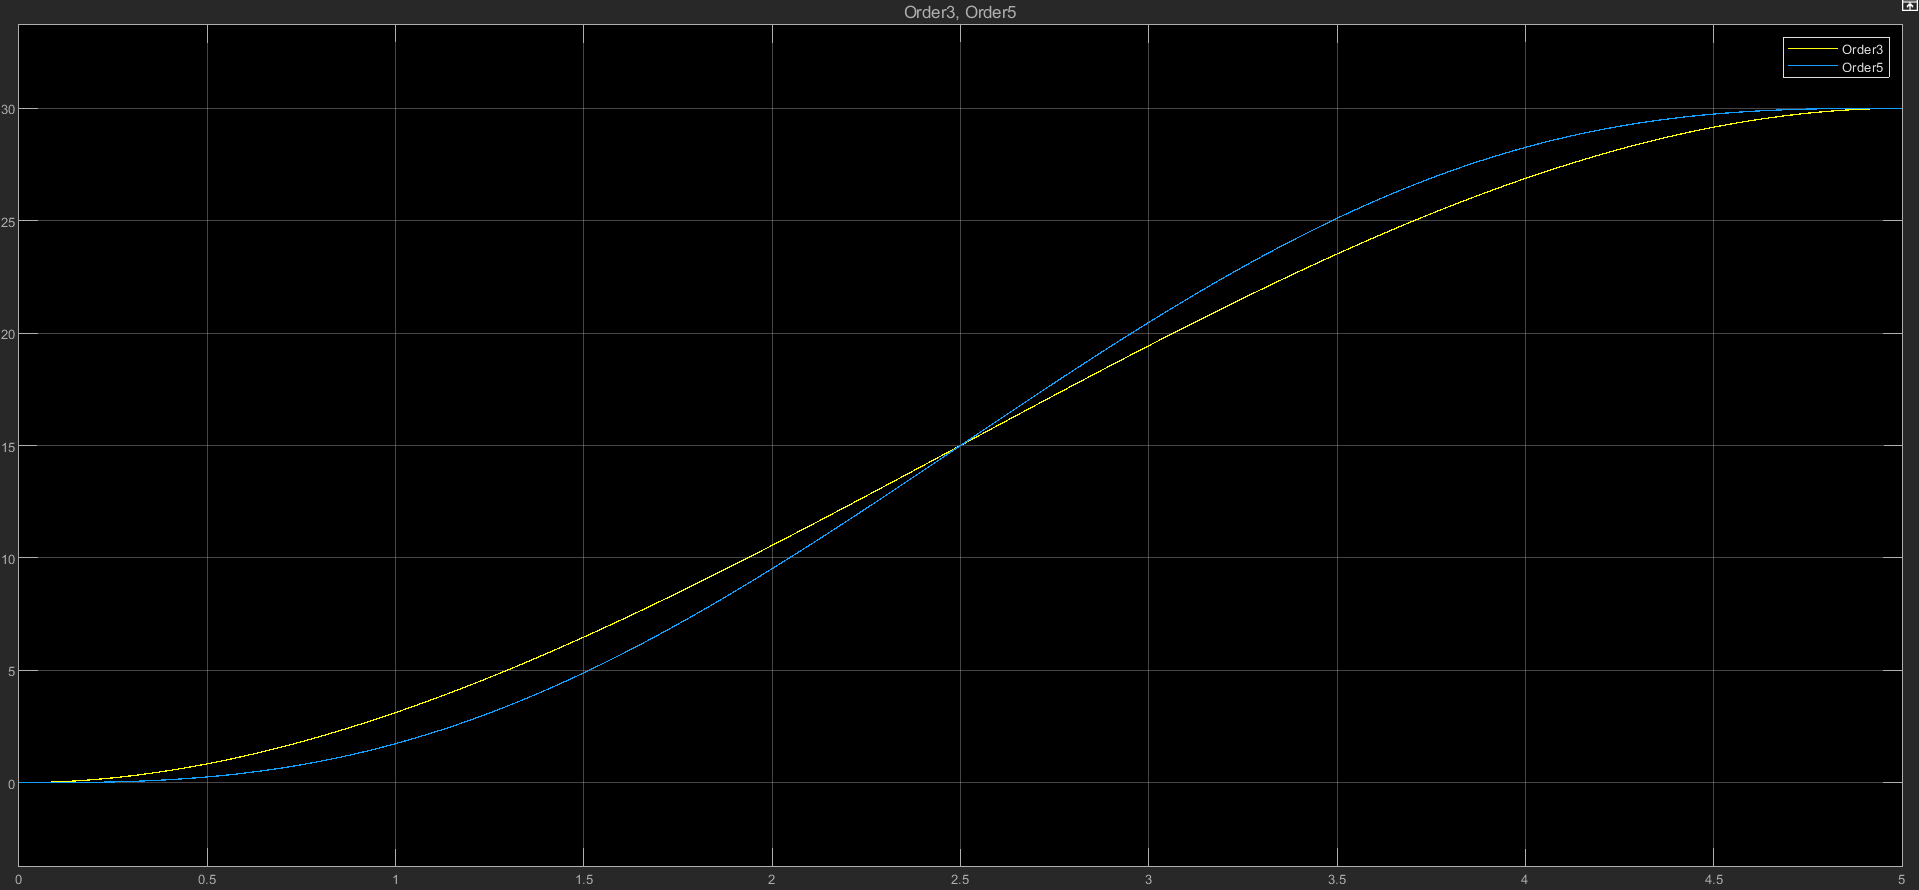
\includegraphics[width=1\linewidth]{../img/16}
	\caption{مسیر مرتبه 3 و 5 برای مفصل تتا4}
	\label{fig:16}
\end{figure}
\begin{figure}[H]
	\centering
	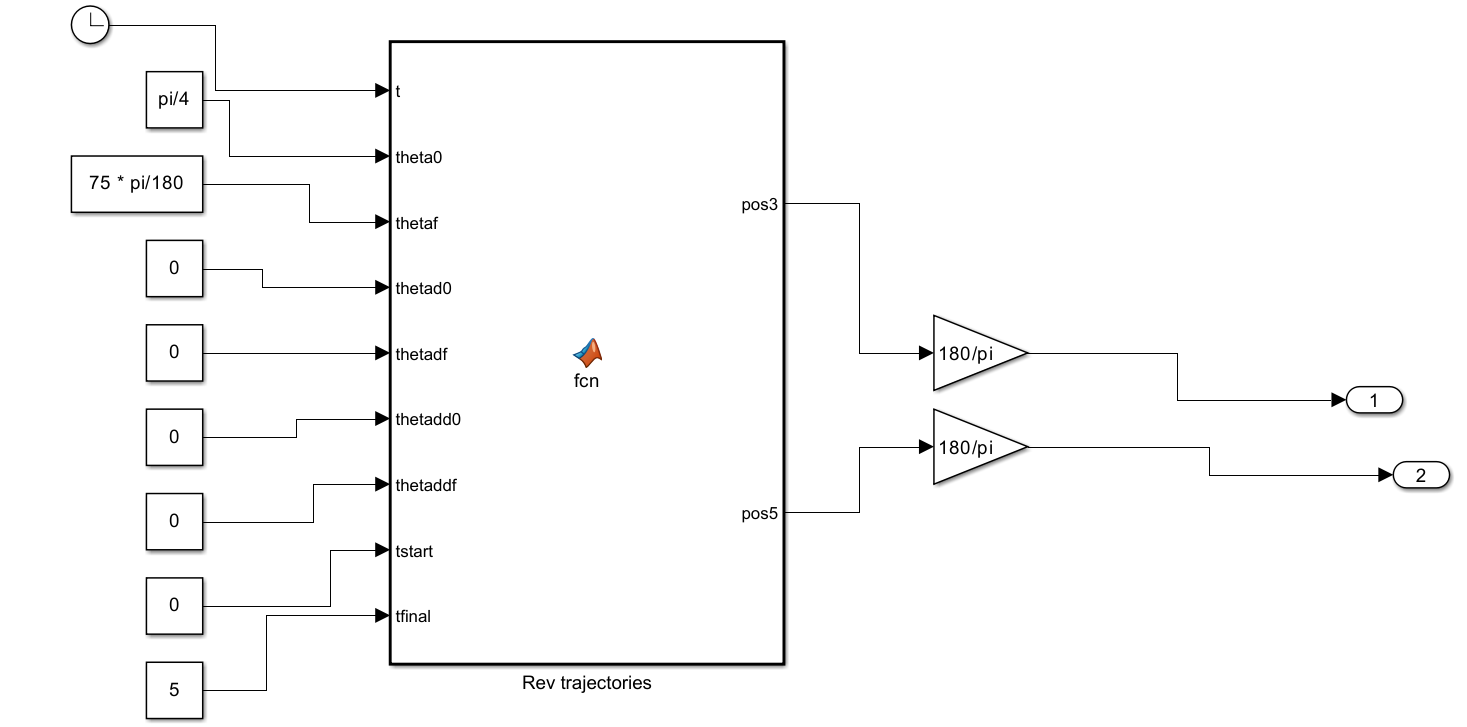
\includegraphics[width=0.7\linewidth]{../img/14}
	\caption{دیاگرام طراحی مسیر مفصل تتا}
	\label{fig:14}
\end{figure}
\begin{figure}
	\centering
	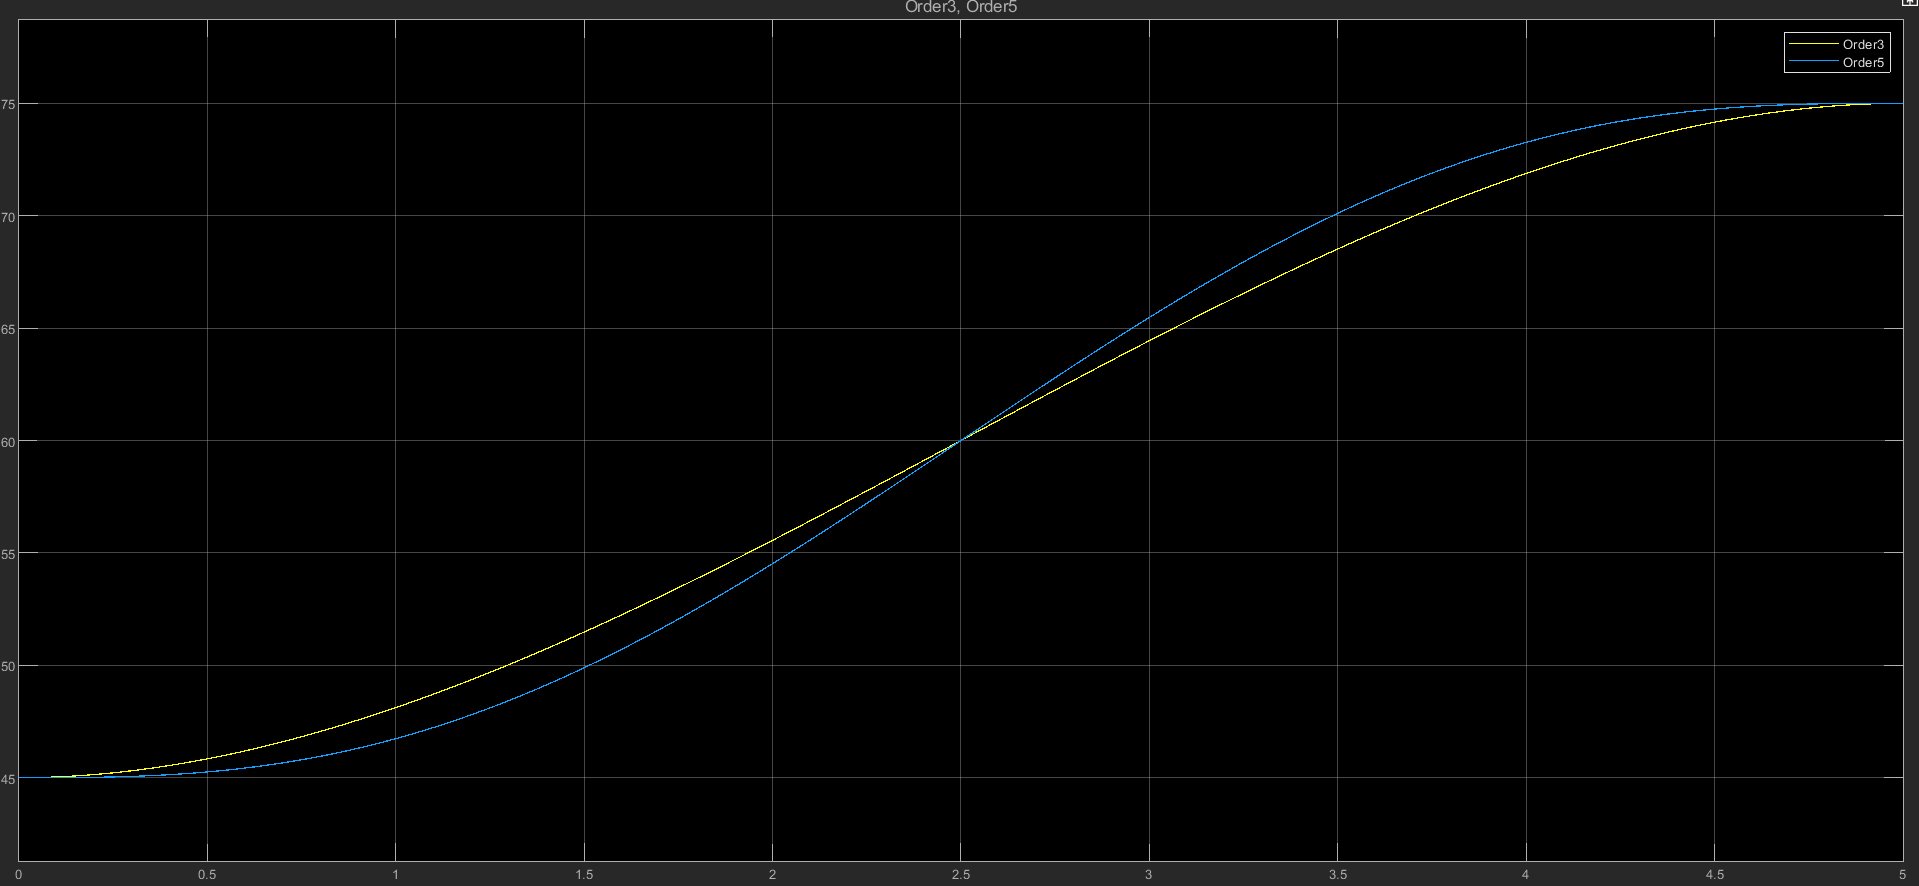
\includegraphics[width=1\linewidth]{../img/17}
	\caption{مسیر مرتبه 3 و 5 برای مفصل تتا}
	\label{fig:17}
\end{figure}
\begin{figure}[H]
	\centering
	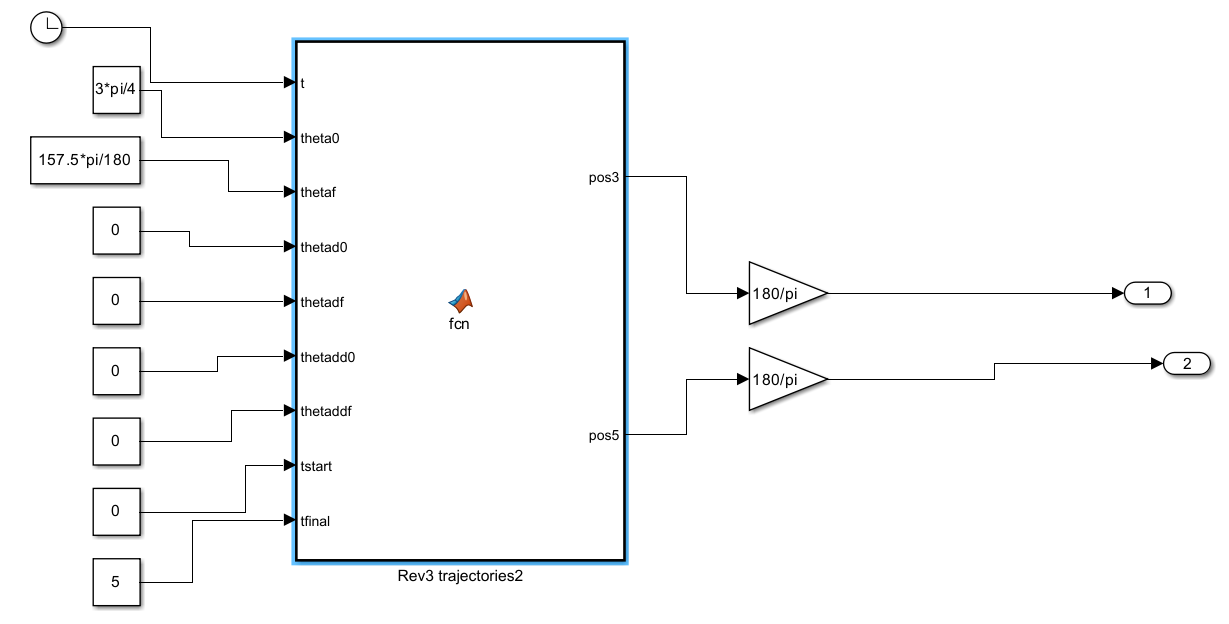
\includegraphics[width=0.7\linewidth]{../img/15}
	\caption{دیاگرام طراحی مسیر مفصل تتا3}
	\label{fig:15}
\end{figure}
\begin{figure}[H]
	\centering
	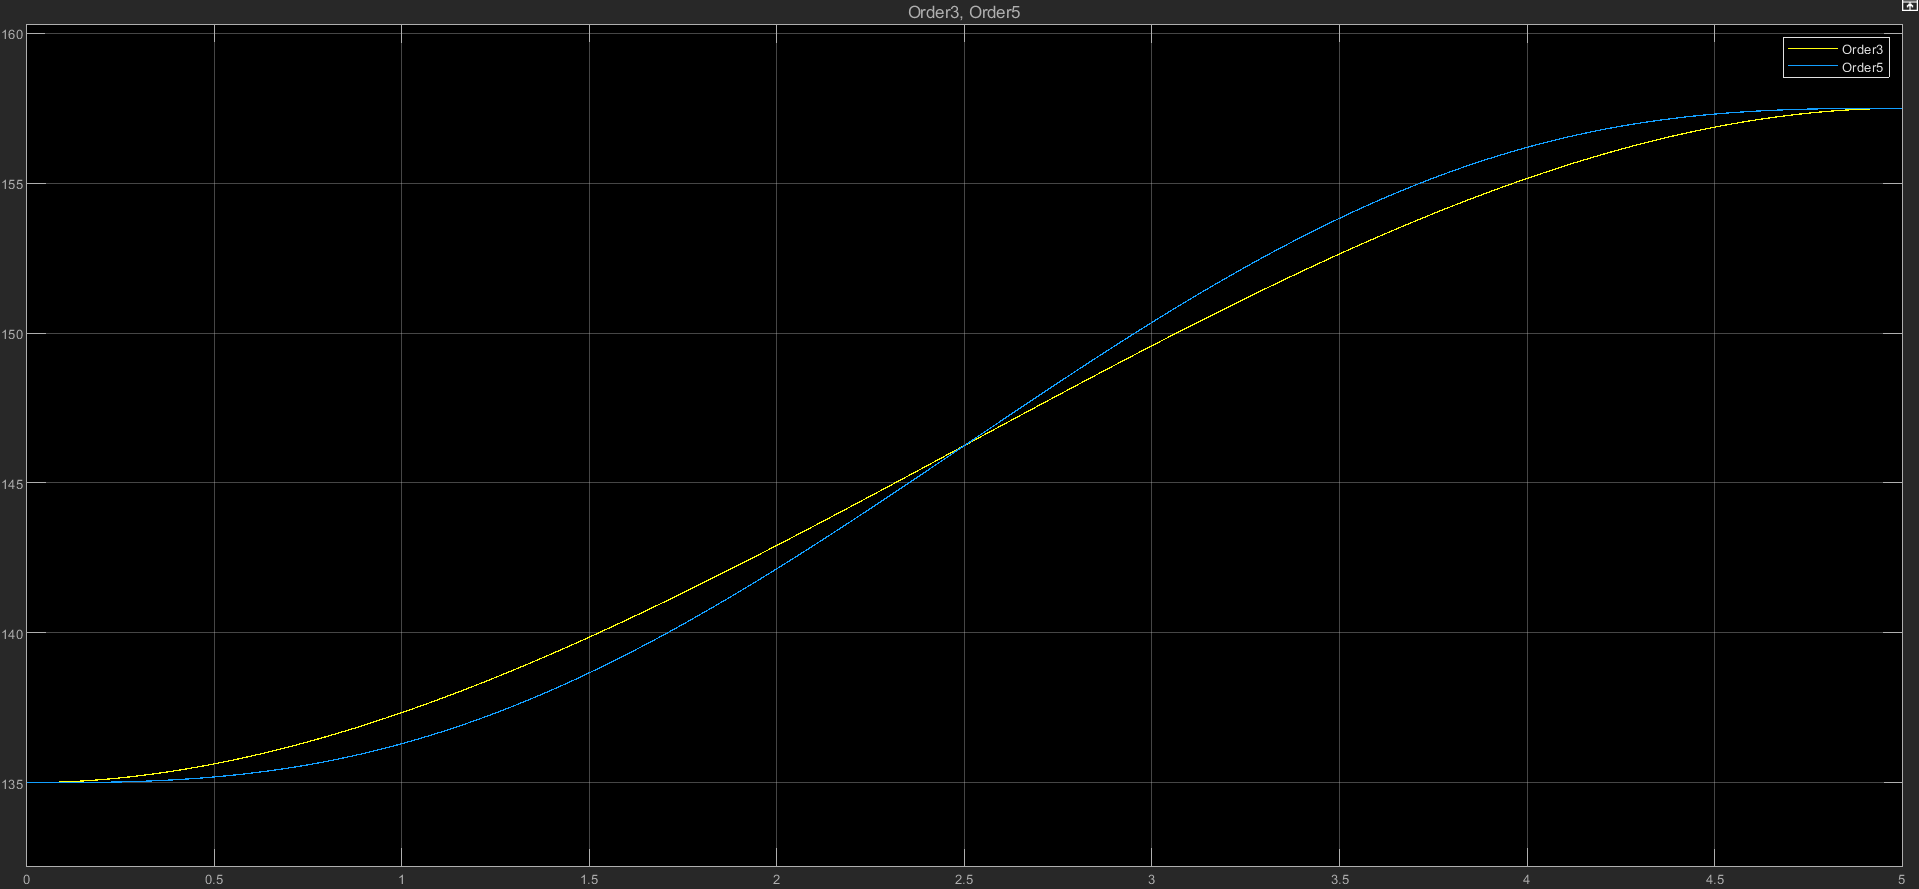
\includegraphics[width=1\linewidth]{../img/18}
	\caption{مسیر مرتبه 3 و 5 برای مفصل تتا3}
	\label{fig:18}
\end{figure}
حال با جایگذاری مسیر مرتبه سوم ایجاد شده توسط این بلوک به عنوان ورودی ربات در شبیه ساز، دیاگرام سیستم به صورت زیر تغییر می کند. 
\begin{figure}[H]
	\centering
	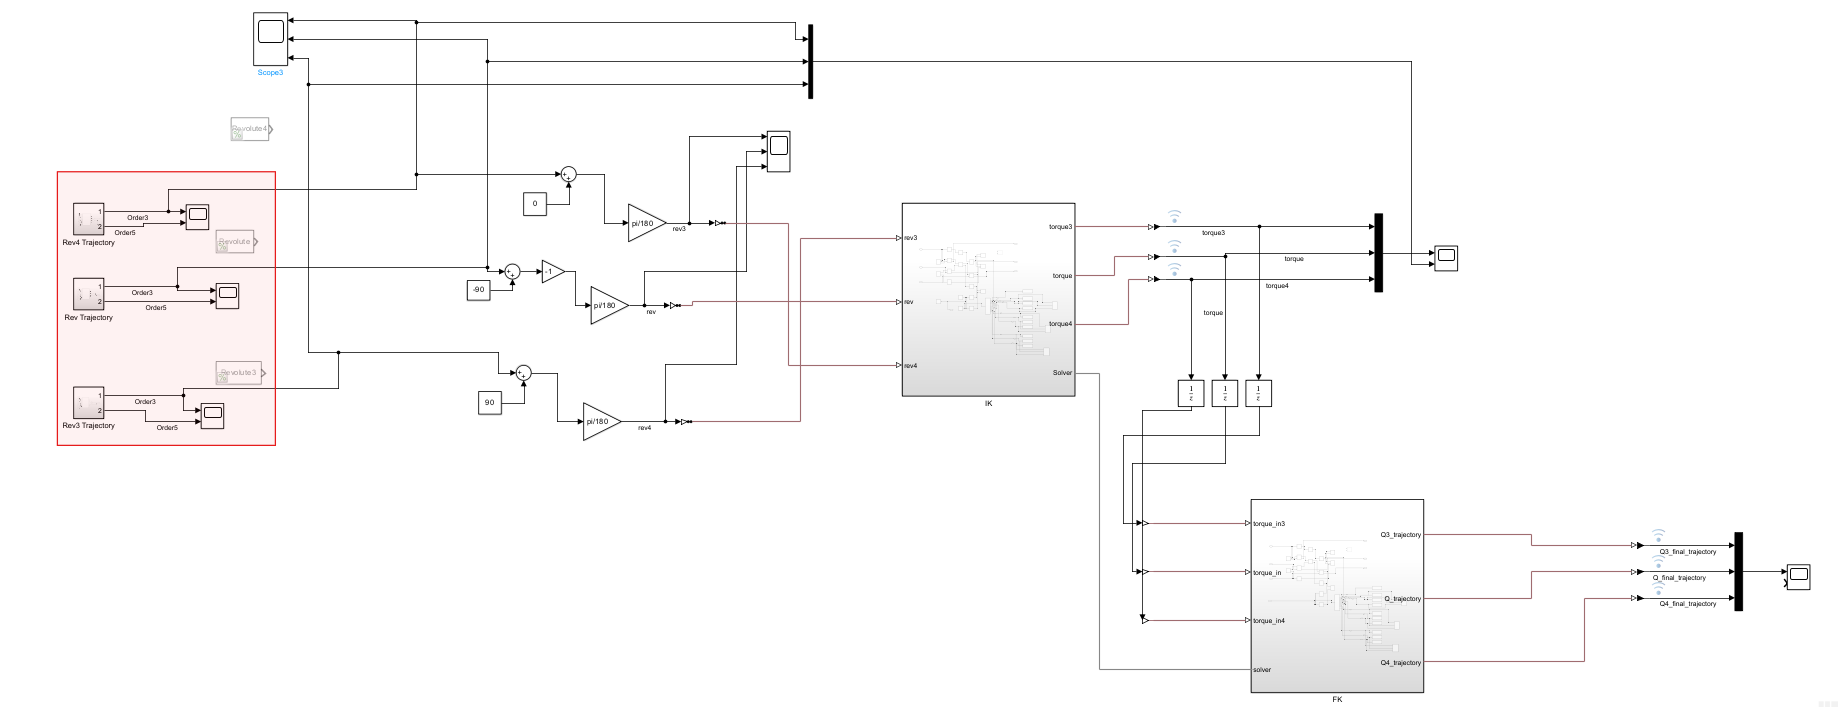
\includegraphics[width=1\linewidth]{../img/19}
	\caption{دیاگرام به همراه بلوک طراحی مسیر}
	\label{fig:19}
\end{figure}
با اعمال این ورودی به بلوک دینامیک وارون سیستم و اندازه گیری مقادیر گشتاور تولید شده، می توانیم نحوه ی عملکرد موتور های سیستم را در بخش های مختلف مسیر مشاهده کنیم.
در نمودار زیر، مسیر حرکتی هر مفصل و گشتاور تولید شده برای آن رسم شده است.

\begin{figure}[H]
	\centering
	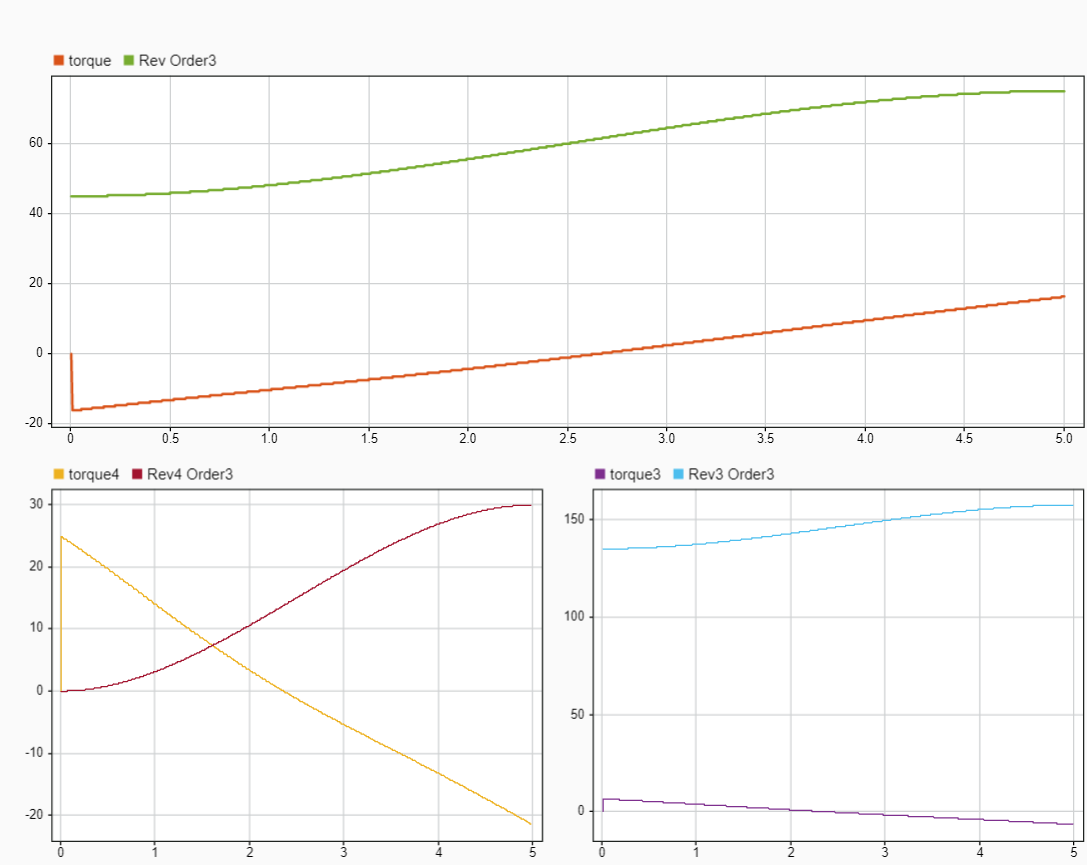
\includegraphics[width=1\linewidth]{../img/20}
	\caption{گشتاور مفصل ها و مسیر ورودی به هر  مفصل}
	\label{fig:20}
\end{figure}
مشاهده می شود که در نقطه ی عطف مسیر هر مفصل، مقدار گشتاور برابر صفر شده و پس از آن، با علامت عکس عمل می کند تا سرعت و شتاب را تا نقطه ی انتهایی به صفر برساند.

برای محاسبه ی توان هر موتور، لازم است مطابق رابطه ی زیر از حاصل ضرب سرعت موتور در گشتاور آن مطابق رابطه ی زیر استفاده کرد. 
\[
P = \tau \cdot \omega
\]
برای اندازه گیری این مقدار در شبیه ساز، ابتدا با مشتق گیری از مسیر داده شده به سیستم، سرعت آن در هر لحظه محاسبه شده و سپس، با ضرب این مقدار در گشتاور اندازه گیری شده، مقدار توان گزارش می شود. 
در نتیجه، دیاگرام این قسمت به صورت زیر به دست می آید. 
\begin{figure}[H]
	\centering
	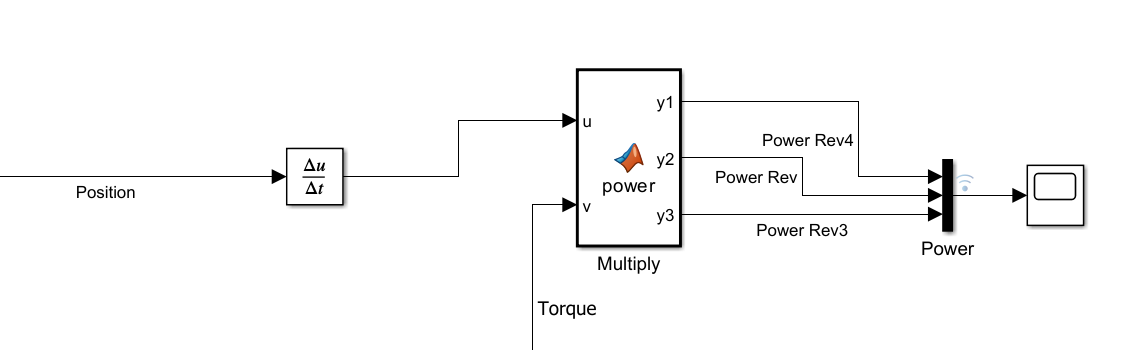
\includegraphics[width=0.7\linewidth]{../img/21}
	\caption{محاسبه توان}
	\label{fig:21}
\end{figure}
با اجرای شبیه سازی، نمودار های توان موتور ها به صورت زیر به دست می آید. 
\begin{figure}[H]
	\centering
	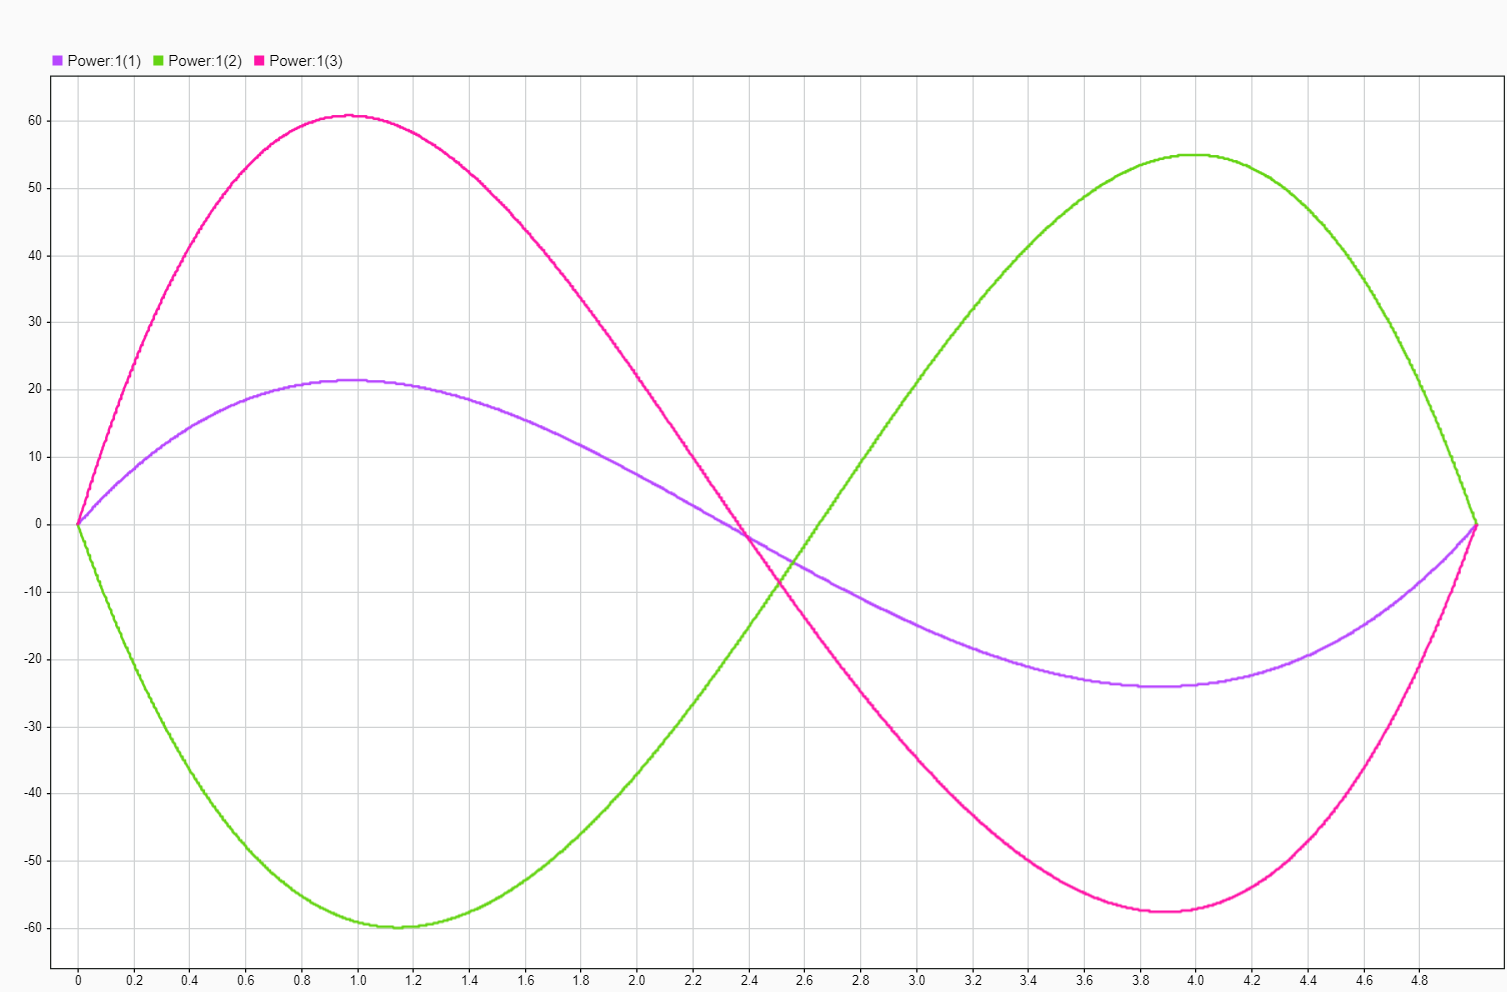
\includegraphics[width=1\linewidth]{../img/22}
	\caption{نمودار توان موتورها}
	\label{fig:22}
\end{figure}

همجنین، برای مقایسه ی توان و گشتاور ها، می توانیم این دو نمودار را در کنار یکدیگر رسم کنیم.
\begin{figure}[H]
	\centering
	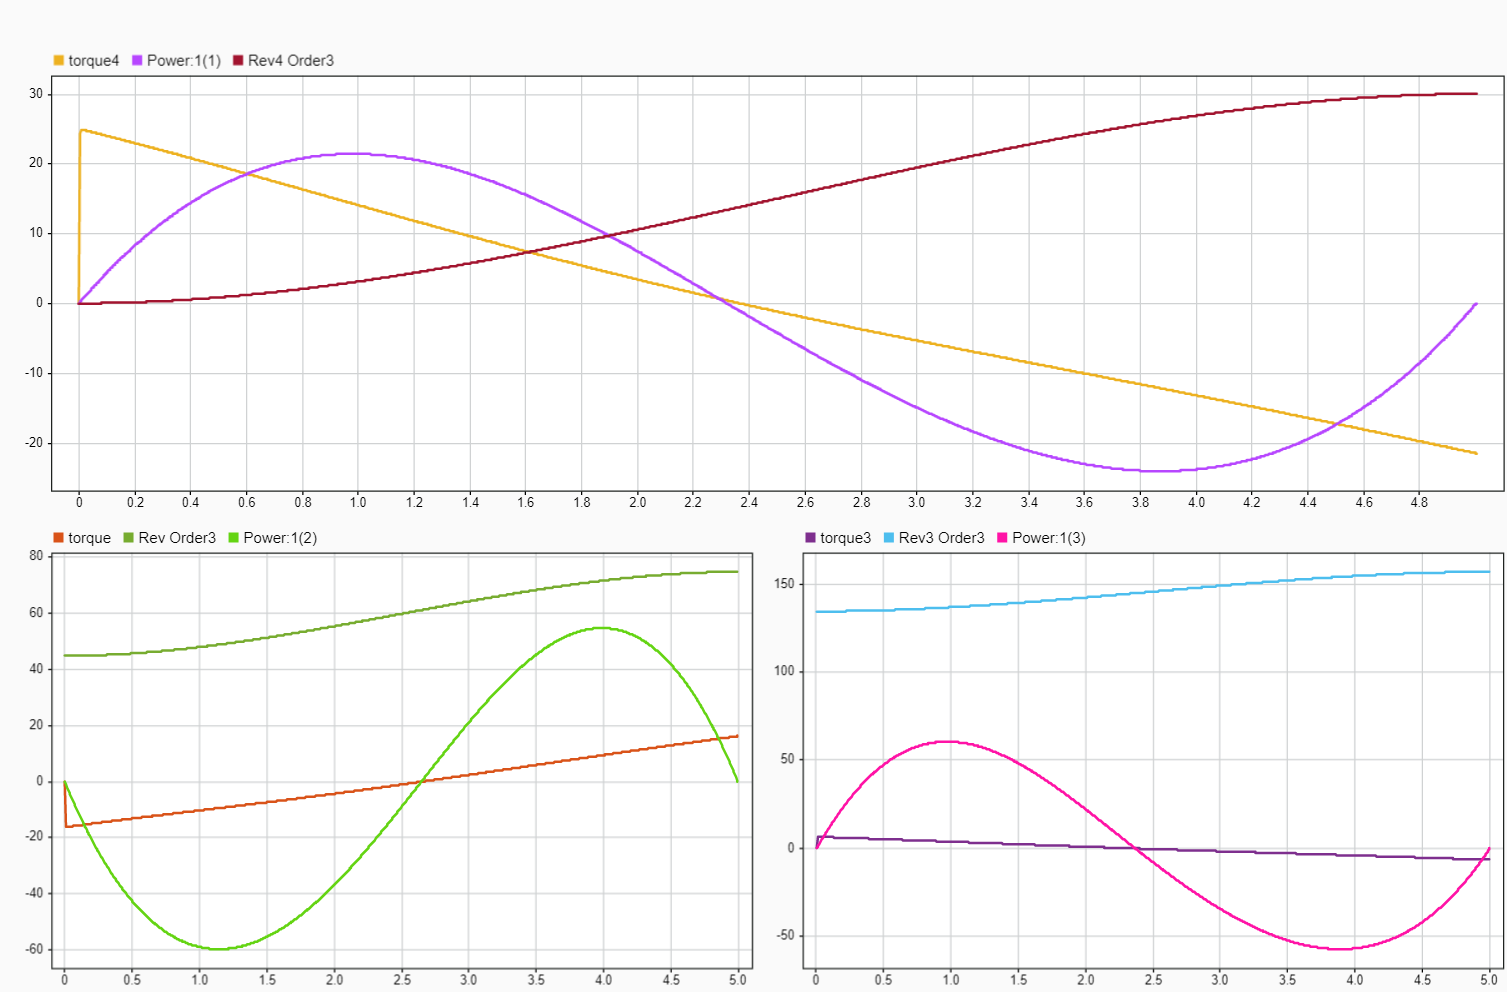
\includegraphics[width=1\linewidth]{../img/23}
	\caption{نمودار توان، گشتاور و مسیر حرکت هر مفصل}
	\label{fig:23}
\end{figure}






















